\documentclass[aer.tex]{subfiles}

\begin{document}

\title{Arbitration}
\maketitle

This document explores arbiters

\tableofcontents


%%%%%%%%%%%%%%%%%%%%%%%%%%%%%%%%%%%%%%%%%%%%%%%%%%%%%%%%%%%%%%%%%%%%%%%%%%%%%%%
\section{2-way Arbiter}

\begin{csp}
*[[#{C0}->C0
  \|#{C1}->C1
 ]]
\end{csp}

\begin{hse}
*[[c0i->c0o+;[~c0i];c0o-
  \|c1i->c1o+;[~c1i];c1o-
 ]]
\end{hse}

\begin{hse}
*[[c0i->c0+;[~c0i];c0-
  \|c1i->c1+;[~c1i];c1-
 ]]

*[[c0->c0o+;[~c0];c0o-
  []c1->c1o+;[~c1];c1o-
 ]]
\end{hse}

Cross-coupled NANDs

\begin{prs2}
c0i & _c1 -> _c0-
~c0i | ~_c1 -> _c0+

c1i & _c0 -> _c1-
~c1i | ~_c0 -> _c1+
\end{prs2}

Filter circuit to ensure $\_c0$ and $\_c1$ are separated by at least a PMOS's threshold voltage

\begin{prs2}
_c1 & ~_c0 -> c0o+
~_c1 | _c0 -> c0o-

_c0 & ~_c1 -> c1o+
~_c0 | _c1 -> c1o-
\end{prs2}

%%%%%%%%%%%%%%%%%%%%%%%%%%%%%%%%%%%%%%%%%%%%%%%%%%%%%%%%%%%%%%%%%%%%%%%%%%%%%%%
\section{N-way Arbiter (N\_ARB) Specification}

The standard arbiter arbitrates between 2 clients and is comprised of 2 cross-coupled NAND gates and a filter circuit for a total of 12 transistors.
In this document, we develop arbiters for N clients.

The N-way arbiter $N\_ARB$ arbitrates between N clients (see Figure~\ref{fig:n_arb}) and is specified by

\begin{figure}
  \centering
  \includegraphics[width=.5\textwidth]{img/transmitter/n_arb.pdf}
  \caption{N\_ARB arbitrates between N children.}
  \label{fig:n_arb}
\end{figure}

\begin{csp}
N_ARB\equiv
  *[[\langle\|n:0..N\-1:#{C`n}->C`n\rangle]]
\end{csp}

\begin{figure}
  \centering
  \includegraphics[width=.5\textwidth]{img/transmitter/n_arb_n_arb_.pdf}
  \caption{N\_ARB decomposed as a binary tree of N\_ARB\_ cells. Here is an N\_ARB instance servicing 4 children. The top N\_ARB\_ cell can simplified to not have a P port or have its P connected back to itself.}
  \label{fig:n_arb_n_arb_}
\end{figure}

We construct the N\_ARB as a binary tree of N\_ARB\_ cells recursively (see Figure~\ref{fig:n_arb_n_arb_}). 

%%%%%%%%%%%%%%%%%%%%%%%%%%%%%%%%%%%%%%%%%%%%%%%%%%%%%%%%%%%%%%%%%%%%%%%%%%%%%%%
\section{Unpipelined N-way Arbiter \label{sec:n_arb_unpipelined}}

This is the arbiter in Rajit's notes to provide mutual exclusion to a shared resource. 
We extend the development with bubble-reshuffled, CMOS-implementable PRS and transistor counts.

\subsubsection*{Transistor accounting}

\begin{center}
    \begin{tabular}{|r|l|l|l|}
    \hline
    component & transistors/component & components/node & transistors/node \\ \hline
    MU\_EX & 20 & 1 & 20 \\ \hline
    PREQ & 18& 1 & 18 \\ \hline
    \multicolumn{3}{|r|}{total transistors/node} & 38 \\ \hline
    \end{tabular}
\end{center}

N\_ARB\_ is constructed as a tree with a 2-way active-low arbiter and 2 associated inverters at the root and N-2 instances of N\_ARB\_. 
Overall, N\_ARB costs $38(N-2)+12+4$ transistors.

\begin{center}
  \begin{tabular}{|r|c|c|c|c|c|c|c|c|c|}
    \hline
    N & 2 & 3 & 4 & 8 & 16 & 32 & 64 & 128 & 256 \\
    \hline
    transistors & 16 & 54 & 92 & 244 & 548 & 1156 & 2372 & 4804 & 9668 \\
    \hline
  \end{tabular}
\end{center}

If the clients expect active high inputs, we'll need N inverters to convert the output of N\_ARB\_ to active high.
In this case, N\_ARB costs $38(N-2)+12+4+2N$ transistors.

\begin{center}
  \begin{tabular}{|r|c|c|c|c|c|c|c|c|c|}
    \hline
    N & 2 & 3 & 4 & 8 & 16 & 32 & 64 & 128 & 256 \\
    \hline
    transistors & 20 & 60 & 100 & 260 & 580 & 1220 & 2500 & 5060 & 10180 \\
    \hline
  \end{tabular}
\end{center}

\subsubsection*{CHP}

We implement this process as a tree of nodes that grant mutually exclusive access to a shared resource.

\begin{csp}
N_ARB_\equiv
*[[#{C`0}->P;C`0
  \|#{C`1}->P;C`1
 ]]
\end{csp}

Client requests are directed up the tree and fulfilled once the parent nodes grant permission. 
There is no pipelining in this design.

We decompose this into concurrent mutual exclusion (MU\_EX) and parent requesting (PREQ) processes.

\begin{csp}
MU_EX\equiv
*[[#{C`0}->Q`0;C`0
  \|#{C`1}->Q`1;C`1
 ]]
\end{csp}
\begin{csp}
PREQ\equiv
*[[#{Q`0}->P;Q`0
  []#{Q`1}->P;Q`1
 ]]
\end{csp}

\subsubsection*{HSE}

MU\_EX
\begin{hse}
*[[c0i->q0o+;[q0i];c0o+;[~c0i];q0o-;[~q0i];c0o-
  \|c1i->q1o+;[q1i];c1o+;[~c1i];q1o-;[~q1i];c1o-
 ]]
\end{hse}

We break out the arbitration.

\begin{hse}
*[[c0i->a0+;[~c0i];a0-
  \|c1i->a1+;[~c1i];a1-
 ]]
*[[a0->q0o+;[q0i];c0o+;[~a0];q0o-;[~q0i];c0o-
  []a1->q1o+;[q1i];c1o+;[~a1];q1o-;[~q1i];c1o-
 ]]
\end{hse}

\noindent PREQ

\begin{hse}
*[[q0i->po+;[pi];q0o+;[~q0i];po-;[~pi];q0o-
  []q1i->po+;[pi];q1o+;[~q1i];po-;[~pi];q1o-
 ]]
\end{hse}

\subsubsection*{PRS}

MU\_EX

\begin{prs2}
~c1o & a0 -> q0o+
c1o | ~a0 -> q0o-

~c0o & a1 -> q1o+
c0o | ~a1 -> q1o-
\end{prs2}

\begin{prs2}
q0i -> c0o+
~q0i -> c0o-

q1i -> c1o+
~q1i -> c1o-
\end{prs2}

\noindent PREQ

\begin{prs2}
q0i | q1i -> po+
~q0i & ~q1i -> po-
\end{prs2}

\begin{prs2}
pi & q0i -> q0o+
~pi -> q0o-

pi & q1i -> q1o+
~pi -> q1o-
\end{prs2}

\begin{center}
  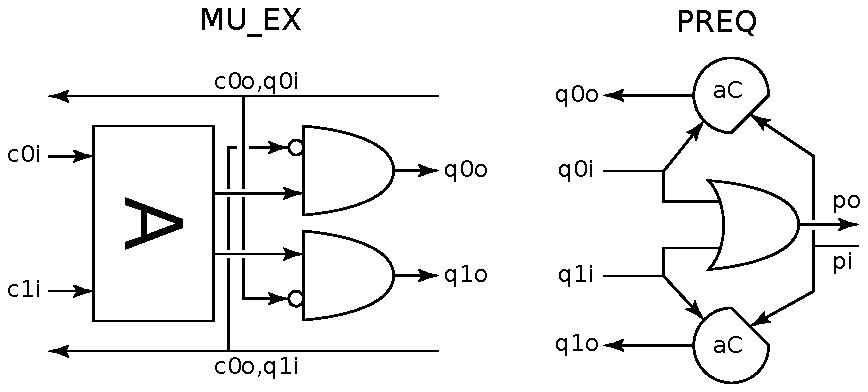
\includegraphics[width=.7\textwidth]{img/standardnwayarbiter.pdf}
\end{center}

\subsubsection*{CMOS-implementable PRS}

\noindent MU\_EX

\begin{prs2}
~c1o & ~_a0 -> q0o+
c1o | _a0 -> q0o-

~c0o & ~_a1 -> q1o+
c0o | _a1 -> q1o-
\end{prs2}

\begin{prs2}
q0i -> c0o+
~q0i -> c0o-

q1i -> c1o+
~q1i -> c1o-
\end{prs2}

\begin{center}
    \begin{tabular}{|r|l|l|}
    \hline
    rule & transistor count & comments \\ \hline
    $\_a[0,1]$ & 12 & 2-way active-low arbiter \\ \hline
    $q[0,1]_o$ & 8 & \\ \hline
    $c[0,1]_o$ & 0 & wires \\ \hline
    \hline total & 20 & \\ \hline
    \end{tabular}
\end{center}

\noindent PREQ

\begin{prs2}
q0i | q1i -> _po-
~q0i & ~q1i -> _po+
\end{prs2}

\begin{prs2}
pi & q0i -> _q0o-
~pi -> _q0o+

pi & q1i -> _q1o-
~pi -> _q1o+
\end{prs2}

\begin{prs2}
_q0o -> q0o-
~_q0o -> q0o+

_q1o -> q1o-
~_q1o -> q1o+
\end{prs2}

\begin{center}
    \begin{tabular}{|r|l|l|}
    \hline
    rule & transistor count & comments \\ \hline
    $\_p_o$ & 4 & \\ \hline
    $\_q[0,1]_o$ & 6 & staticizers on $q[0,1]_o$ \\ \hline
    $q[0,1]_o$ & 8 & staticizes $\_q[0,1]_o$ \\ \hline
    \hline total & 18 & \\ \hline
    \end{tabular}
\end{center}

\subsubsection*{Notes}

That this implementation does not gaurantee mutual exclusion of the output signals between clients across leaves of the arbiter tree for more than 2 clients. 
For example, consider the 4 client case with inputs 0 and 3 high. The N-way arbiter selects 0 first. 0 clears its input. The parent arbiter node clears $p_i$, and the 0 output will clear sometime in the future. 
However, because $p_i$ has cleared, the parent node is free to select the other child and can complete the full communication with 3 even before the 0 output clears. 
To fix this, the outputs would have to mutually exclude the requests of all other clients across the leaf nodes.

%%%%%%%%%%%%%%%%%%%%%%%%%%%%%%%%%%%%%%%%%%%%%%%%%%%%%%%%%%%%%%%%%%%%%%%%%%%%%%%
\section{Alternative Unpipelined N-way Arbiter}

Here's an alternative to the previous, unpipelined design.

\subsubsection*{Transistor accounting}

N\_ARB\_ is constructed as a tree with a 2-way arbiter at the root and $N-2$ instances of N\_ARB\_. Overall, N\_ARB\ costs $40(N-2)+12$ transistors.

\begin{center}
  \centering
  \begin{tabular}{|r|c|c|c|c|c|c|c|c|c|}
    \hline
    N & 2 & 3 & 4 & 8 & 16 & 32 & 64 & 128 & 256 \\
    \hline
    transistors & 12 & 52 & 92 & 252 & 572 & 1212 & 2492 & 5052 & 10172 \\
    \hline
  \end{tabular}
\end{center}

\subsubsection*{CHP}

\begin{csp}
N_ARB_\equiv
  *[[C0\star\!P;C0\star\!P
    \|C1\star\!P;C1\star\!P]]
\end{csp}

\subsubsection*{HSE}

\begin{hse}
*[[c0i->c0+;[~c0i];c0-
  \|c1i->c1+;[~c1i];c1-]]
*[[c0->po+;[pi];c0o+;[~c0];po-;[~pi];c0o-
  []c1->po+;[pi];c1o+;[~c1];po-;[~pi];c1o-]]
\end{hse}

\subsubsection*{PRS}

\begin{prs2}
c0 & ~c1o | c1 & ~c0o -> po+
~c0 & c0o | ~c1 & c1o -> po-
\end{prs2}

\begin{prs2}
pi & c0 & ~c1o -> c0o+
~pi -> c0o-

pi & c1 & ~c0o -> c1o+
~pi -> c1o-
\end{prs2}

\subsubsection*{CMOS-implementable PRS}

\noindent A standard 2-input arbiter takes in $c0_i$ and $c1_i$ to generate $c0$ and $c1$.

\begin{prs2}
c0 & _c1o | c1 & _c0o -> _po-
~c0 & ~_c0o | ~c1 & ~_c1o -> _po+
\end{prs2}

\begin{prs2}
pi & c0 & _c1o -> _c0o-
~pi -> _c0o+

pi & c1 & _c0o -> _c1o-
~pi -> _c1o+
\end{prs2}

\begin{prs2}
_po -> po-
~_po -> po+

_c0o -> c0o-
~_c0o -> c0o+

_c1o -> c1o-
~_c1o -> c1o+
\end{prs2}

accounting:

\begin{center}
    \begin{tabular}{|r|l|l|}
    \hline
    rule & transistor count & comments \\ \hline
    $\_p_o$ & 8 & \\ \hline
    $c[0,1]$ & 12 & standard 2-way arbiter \\ \hline
    $\_c[0,1]_o$ & 8 & \\ \hline
    $p_o$ & 4 & staticizer \\ \hline
    $c[0,1]_o$ & 8 & staticizer \\ \hline
    \hline total & 40 & \\ \hline
    \end{tabular}
\end{center}

%%%%%%%%%%%%%%%%%%%%%%%%%%%%%%%%%%%%%%%%%%%%%%%%%%%%%%%%%%%%%%%%%%%%%%%%%%%%%%%
\section{Greedy but Fair N-way Arbiter}

In this design, 

\begin{csp}
N\_ARB\_ \equiv H\_ARB
\end{csp}

N\_ARB will be constructed from $N-1$ H\_ARB instances. so N\_ARB requires approximately $110(N-1)$ transistors.

\begin{center}
  \begin{tabular}{|r|c|c|c|c|c|c|c|c|c|}
    \hline
    N & 2 & 3 & 4 & 8 & 16 & 32 & 64 & 128 & 256 \\
    \hline
    transistors & 110 & 220 & 330 & 770 & 1650 & 3410 & 6930 & 13970 & 28050 \\
    \hline
  \end{tabular}
\end{center}

Note that the basic, 2-input arbiter only requires 12 transistors, almost tenfold less than a 2-input N\_ARB. \\
We might require N inverters to interface with the client's output. 
We will need inverter to connect the top of the tree back to itself, 
so in the worst case we'll need $110(N-1)+2N+2=112(N-1)+4$ transistors.

%%%%%%%%%%%%%%%%%%%%%%%%%%%%%%%%%%%%
\subsection{Heirarchical arbiter H\_ARB}

H\_ARB coordinates with its parent (another H\_ARB instance) and arbitrates between two children. 
With ports

\begin{tabular}[]{rl}
$C0$ & child 0 port \\
$C1$ & child 1 port \\
$P$ & parent port \\
\end{tabular} \\

\noindent H\_ARB is specified by

\begin{csp}
H_ARB\equiv
  *[[#{C`0}|#{C`1}->P;
    [#{C`0}->C`0;C`0\|~#{C`0}->skip];
    [#{C`1}->C`1;C`1\|~#{C`1}->skip];P]]
\end{csp}

When a child request arrives, H\_ARB sends a request to its parent. When the parent gives permission to go ahead, H\_ARB checks the first child and then the second child. During each check, H\_ARB services the child if its request is present. Otherwise, H\_ARB skips and moves on. After checking the children, H\_ARB releases its parent.

H\_ARB implements a greedy yet fair arbitration algorithm. H\_ARB is greedy because it can service both children for a single request to the parent. H\_ARB is fair because it will service each child at most once for each request to the parent. 

\begin{figure}
  \centering
  \includegraphics[width=.5\textwidth]{img/transmitter/arb_h_detail.pdf}
  \caption{$H\_ARB$ decomposition. Dotted line indicates wire used for probing only.}
  \label{fig:h_arb_detail}
\end{figure}

We decompose H\_ARB into a control cell $CTRL$ and two child arbitration cells $C\_ARB$ as in Figure~\ref{fig:h_arb_detail}.

\begin{csp}
H\_ARB\equiv\!CTRL\pll\!C_ARB\pll\!C_ARB
\end{csp}

\begin{figure}
  \centering
  \includegraphics[width=.7\textwidth]{img/transmitter/H_ARB_bubble_reshuffled.pdf}
  \caption{H\_ARB after bubble reshuffling. Ports are expanded and inverters introduced by bubble reshuffling are shown.}
  \label{fig:h_arb_bubbled}
\end{figure}

\noindent Bubble reshuffling $CTRL$ and $C\_ARB$ yields the H\_ARB shown in Figure~\ref{fig:h_arb_bubbled}.

\noindent Accounting:

\begin{center}
    \begin{tabular}{|r|l|l|l|}
    \hline
    component & transistors/component & components/H\_ARB & transistors/H\_ARB \\ \hline
    CTRL & 36 & 1 & 36 \\ \hline
    C\_ARB & 34 & 2 & 68 \\ \hline
    inverters & 2 & 3 & 6 \\ \hline
    \hline \multicolumn{3}{|r|}{total transistors/H\_ARB} & 110 \\ \hline
    \end{tabular}
\end{center}

%%%%%%%%%%%%%%%%%%%%%%%%%%%%%%%%%%%%%%%
\subsection{Control cell CTRL}
CTRL sequences communications with the parent of H\_ARB and the child arbiters.
CTRL has ports

\begin{tabular}[]{rl}
$P$ & parent port \\
$S_0$ & child arbiter 0 port \\
$S_1$ & child arbiter 1 port \\
\end{tabular} \\

\subsubsection*{CHP}

\begin{csp}
CTRL\equiv
  *[[#{C`0}|#{C`1}->P;S`0;S`0;S`1;S`1;P]]
\end{csp}

\noindent where 

\begin{tabular}[]{rl}
  $C_0$ & probes child 0 \\
  $C_1$ & probes child 1 \\
  $P$ & communicates with the parent \\
  $S_0$ & communicates with the child 0 arbiter \\
  $S_1$ & communicates with the child 1 arbiter \\
\end{tabular} \\ \\

\subsubsection*{HSE}

\noindent Directly translating the CHP,

\begin{hse}
CTRL\equiv
  *[[c0i|c1i];po+;[pi];
    s0o+;[s0i];s0o-;[~s0i];
    s1o+;[s1i];s1o-;[~s1i];
    po-;[~pi]]
\end{hse}

\noindent There are 3 indistinguishable states--after $[p_i]$, after $s0_o\!\downarrow$, and after $s1_o\!\downarrow$. The correct operation of CTRL precludes reshuffling to break symmetry, so we use 2 state variables to distinguish betwen the 3 states.

\begin{hse}
CTRL\equiv
  *[[c0i|c1i];po+;[pi];x-;
    s0o+;[s0i];y-;s0o-;[~s0i];
    s1o+;[s1i];x+;s1o-;[~s1i];
    po-;[~pi];y+]
\end{hse}

\subsubsection*{PRS}

\begin{prs2}
(c0i | c1i) & y -> po+
~s1i & x & ~y -> po-
\end{prs2}

\begin{prs2}
s1i & ~y -> x+
pi & y -> x-

~pi -> y+
s0i -> y-
\end{prs2}

\begin{prs2}
~x & y -> s0o+
x | ~y -> s0o-

~s0i & ~x & ~y -> s1o+
x -> s1o-
\end{prs2}

\noindent after bubble reshuffling

\begin{prs2}
(~_c0i | ~_c1i) & ~_y -> po+
_s1i & x & _y -> po-

po -> _po-
~po -> _po+
\end{prs2}

\begin{prs2}
~x & ~_y -> s0o+
x | _y -> s0o-

~s0i & ~x & ~y -> s1o+
x -> s1o-
\end{prs2}

\begin{prs2}
~_s1i & ~y -> x+
pi & y -> x-

~pi -> y+
s0i -> y-
\end{prs2}

\noindent Transistor accounting:

\begin{center}
    \begin{tabular}{|r|l|l|}
    \hline
    rule & transistor count & comments \\ \hline
    $p_o$ & 6 & \\ \hline
    $\_p_o$ & 4 & includes staticizer for $p_o$ \\ \hline
    $s0_o$ & 4 & \\ \hline
    $s1_o$ & 8 & \\ \hline
    $x$ & 8 & \\ \hline
    $y$ & 6 & \\ \hline
    \hline total & 36 & \\ \hline
    \end{tabular}
\end{center}

%%%%%%%%%%%%%%%%%%%%%%%%%%%%%%%%%%%%%%%
\subsection{Child arbiter C\_ARB}
C\_ARB determines whether or not a child's request is present when called upon by CTRL.

\subsubsection*{CHP}

\begin{csp}
C_ARB\equiv
  *[[#C->S;C;C;S
    \|#S->S;S]]
\end{csp}

\noindent where 

\begin{tabular}[]{rl}
  $C$ & communicates with the child \\ 
  $S$ & communicates with $CTRL$ \\
\end{tabular} \\ \\

We arbitrate between requests from the child, $\overline{C}$, and 
requests from CTRL, $\overline{S}$. If a child request is present, the arbiter is biased towards selecting the child because $S$ requests will not arrive until CTRL has obtained permission from the parent. Although small, there is a chance that a child's request will be skipped on a given iteration of CTRL, but the weakly fair assumption ensures that the child will be serviced eventually.

\noindent If the arbitration selects the child request $\overline{C}$, C\_ARB

\begin{tabular}[]{rl}
  $S$ & waits for and acknowledge CTRL's request \\
  $C$ & signals the child to proceed \\
  $C$ & waits for the child to complete \\
  $S$ & releases CTRL so it can move on \\
\end{tabular} \\ \\

\noindent If the arbitration selects CTRL's request $\overline{S}$, C\_ARB

\begin{tabular}[]{rl}
  $S$ & waits for and acknowledge CTRL's request \\
  $S$ & releases CTRL so it can move on \\
\end{tabular} \\ \\

\noindent which is a simple 4-phase handshake. Note that $S$ is shared between the two branches.

\subsubsection*{HSE}

\noindent Directly translating the CHP,

\begin{hse}
*[[ci->[si];so+;co+;[~ci];co-;[~si];so-
  \|si->so+;[~si];so-]]
\end{hse}

\noindent We introduce intermediate variables $c$ and $s$ to represent the arbitration,

\begin{hse}
*[[ci->c+;[si];so+;co+;[~ci];c-;co-;[~si];so-
  \|si->s+;so+;[~si];s-;so-]]
\end{hse}

\noindent and break out the arbitration into a separate process

\begin{hse}
*[[ci->c+;[~ci];c-
  \|si->s+;[~si];s-]]
*[[c->[si];so+;co+;[~c];co-;[~si];so-
  []s->so+;[~s];so-]]
\end{hse}

\noindent Note that the $c$ branch of the select statement uses $s_i$ and not $s$. In addition, as soon as $c_o$ goes high, $c_i$ could clear before $s_i$, which would allow the arbitration process to complete its $c_i$ branch and select the $s_i$ branch while the $c$ branch is still in progress. We thus wait for $s_i$ to clear before communicating with the child.

\begin{hse}
*[[ci->c+;[~ci];c-
  \|si->s+;[~si];s-]]
*[[c->[si];so+;[~si];co+;[~c];co-;so-
  []s->so+;[~s];so-]]
\end{hse}

\noindent After $co\!\downarrow$, the child could raise its request again ($c_i$) and greedily hold the circuit in a loop servicing the child. We break this loop by releasing CTRL ($s_o\!\downarrow$) before releasing the child.

\begin{hse}
*[[ci->c+;[~ci];c-
  \|si->s+;[~si];s-]]
*[[c->[si];so+;[~si];co+;[~c];so-;co-
  []s->so+;[~s];so-]]
\end{hse}

\noindent Note that $s_o$ is shared between both branches of selection statement. This sharing results in interfering production rules for $s_o$, so we introduce intermediate values $cs_o$ and $ss_o$ and merge them in a third concurrent process.

\begin{hse}
*[[ci->c+;[~ci];c-
  \|si->s+;[~si];s-]]\pll
*[[c->[si];cso+;[~si];co+;[~c];cso-;co-
  []s->sso+;[~s];sso-]]\pll
*[[cso->so+;[~cso];so-]
  []sso->so+;[~sso];so-]
\end{hse}

\subsubsection*{PRS}

\noindent $s_i$ and $c_i$ are inputs to a standard 2-input arbiter, which outputs $s$ and $c$.

\begin{prs2}
c & si & ~sso -> cso+
~c -> cso-

s & ~co -> sso+
~s | co -> sso-
\end{prs2}

\begin{prs2}
~si & cso -> co+
si | ~cso -> co-

cso | sso -> so+
~cso & ~sso -> so-
\end{prs2}

\noindent after bubble reshuffling

\begin{prs2}
~_c & ~_si & ~sso -> cso+
_c -> cso-

~_s & ~co -> sso+
_s | co -> sso-
\end{prs2}

\begin{prs2}
_si & cso -> _co-
~_si | ~cso -> _co+

_co -> co-
~_co -> co+

cso | sso -> _so-
~cso & ~sso -> _so+
\end{prs2}

\noindent where $\_s$ and $\_c$ come from an active-low 2-input arbiter with inputs $\_s_i$ and $\_c_i$. 

\noindent Transistor accounting:

\begin{center}
    \begin{tabular}{|r|l|l|}
    \hline
    rule & transistor count & comments \\ \hline
    $\_[s,c]$ & 12 & 2-input arbiter \\ \hline
    $cs_o$ & 8 & \\ \hline
    $ss_o$ & 4 & \\ \hline
    $\_c_o$ & 4 & \\ \hline
    $c_o$ & 2 & \\ \hline
    $\_s_o$ & 4 & \\ \hline
    \hline total & 34 & \\ \hline
    \end{tabular}
\end{center}

%%%%%%%%%%%%%%%%%%%%%%%%%%%%%%%%%%%%%%%%%%%%%%%%%%%%%%%%%%%%%%%%%%%%%%%%%%%%%%%
\section{Greedy but Fair N-way Arbiter using Tree/Ring Sequencing}

The tree is built from NODEs. 
The leaves of the tree service requests from $N$ clients.

\subsubsection*{Accounting}

NODES cost 30$K$+18 transistors, where $K$ is the radix of the tree.

\begin{center}
    \begin{tabular}{|r|l|}
    \hline
    Configuration & transistors \\ \hline
    $K$-ary tree & $(30K+18)\frac{N-1}{K-1}$ \\ \hline
    Flat ring & $30N+18$ \\ \hline
    Binary tree & $78(N-1)$ \\ \hline
    4-ary tree & $46(N-1)$ \\ \hline
    \end{tabular}
\end{center}

%%%%%%%%%%%%%%%%%%%%%%%%%%%%%%%%%%%%%%%%%%%%%%%%%%%%%%%%%%%%
\subsection{NODE}

For a binary tree,

\begin{csp}
*[[#{C`0}|#{C`1}];P\*(
  [#{C`0}->C`0;C`0\|~#{C`0}->skip];
  [#{C`1}->C`1;C`1\|~#{C`1}->skip])
 ]
\end{csp}

\noindent
For a $K$-ary tree,

\begin{csp}
*[[\langle|k:K:#{C`k}\rangle];
  P\*\langle;k:K:[#{C`0}->C`0;C`0\|~#{C`0}->skip]\rangle
 ]]
\end{csp}

\noindent
We decompose NODE into PRODUCER and CONSUMER processes.

\subsubsection*{Accounting}

\begin{center}
    \begin{tabular}{|r|l|l|l|}
    \hline
    component & transistors/component & components/NODE & transistors/NODE \\ \hline
    PRODUCER & 18+$K$ & 1 & 18+$K$ \\ \hline
    CONSUMER & 29 & $K$ & 29$K$ \\ \hline
    \hline \multicolumn{3}{|r|}{total transistors/NODE} & 30$K$+18 \\ \hline
    \end{tabular}
\end{center}

%%%%%%%%%%%%%%%%%%%%%%%%%%%%%%%%%%%%%%%%%%%%%%%%%%%%%%%%%%%%
\subsection{PRODUCER}

PRODUCER produces parent requests upon sensing child requests
and sequences between CONSUMERs.
For a binary tree,

\begin{csp}
*[[#{C`0}|#{C`1}];P\*\langle\*K:k:S`k\rangle]]
\end{csp}

\noindent
For a $K$-ary tree,

\begin{csp}
*[[\langle|K:k:#{C`k}\rangle];P\*\langle\*K:k:S`k\rangle]]
\end{csp}

\noindent 
We decompose PRODUCER into CTRL and SEQ.

\subsubsection*{Accounting}

\begin{center}
    \begin{tabular}{|r|l|l|l|}
    \hline
    component & transistors/component & components/PRODUCER & transistors/PRODUCER \\ \hline
    CTRL & 18+$K$ & 1 & 18+$K$ \\ \hline
    SEQ & 0 & 1 & 0 \\ \hline
    \hline \multicolumn{3}{|r|}{total transistors/PRODUCER} & 18+$K$ \\ \hline
    \end{tabular}
\end{center}

%%%%%%%%%%%%%%%%%%%%%%%%%%%%%%%%%%%%%%%%%%%%%%%%%%%%%%%%%%%%
\subsection{CTRL}

CTRL relays the child requests to the parent 
and initiates the sequencing between CONSUMERS.

\subsubsection*{CHP}

For a binary tree,

\begin{csp}
*[[#{C`0}|#{C`1}];P\*S]
\end{csp}

\noindent For a $K$-ary tree,

\begin{csp}
*[[\langle|K:k:#{C`k}\rangle];P\*S]
\end{csp}

\subsubsection*{HSE}

For a binary tree,

\begin{hse}
*[[pe];[c0r|c1r];x-;
  pr+;[~pe];
  sr+;[sa];x+;sr-;[~sa];
  pr-]
\end{hse}

\subsubsection*{PRS}

\begin{prs2}
pe & (c0r | c1r) -> x-
sa -> x+
\end{prs2}

\begin{prs2}
~x | sa -> pr+
x & ~sa -> pr-
\end{prs2}

\begin{prs2}
~x & ~pe -> sr+
x | pe -> sr-
\end{prs2}

\subsubsection*{CMOS-implementable PRS}

\begin{prs2}
pe & (c0r | c1r) -> x-
~_sa -> x+
\end{prs2}

\begin{prs2}
~x | ~_sa -> pr+
x & _sa -> pr-
\end{prs2}

\begin{prs2}
~x & ~pe -> sr+
x | pe -> sr-
\end{prs2}

\begin{prs2}
_pe -> pe-
~_pe -> pe+

sa -> _sa-
~sa -> _sa+
\end{prs2}

\subsubsection*{Accounting}

\begin{center}
    \begin{tabular}{|r|l|l|}
    \hline
    rule & transistor count & comments \\ \hline
    $x$ & 2+$K$+4 & \\ \hline
    $pr$ & 4 & \\ \hline
    $sr$ & 4 & \\ \hline
    $pe$ & 2 & \\ \hline
    $_sa$ & 2 & \\ \hline
    \hline total & 18+$K$ & \\ \hline
    \end{tabular}
\end{center}

%%%%%%%%%%%%%%%%%%%%%%%%%%%%%%%%%%%%%%%%%%%%%%%%%%%%%%%%%%%%
\subsection{SEQ}

SEQ sequences through the consumers.

\subsubsection*{CHP}

In general,

\begin{csp}
SEQ(K)\equiv
*[SP\*\langle\*k:K:SC`k\rangle]
\end{csp}

\noindent
For a binary tree,

\begin{csp}
*[SP\*SC`0\*SC`1]
\end{csp}

\noindent
We build a $K$-way sequencer as $K'$-way sequencer tree defined recursively as

\begin{csp}
SEQ(K)\equiv\!SEQ(K')\pll\langle\pll\!k':K'\-1:SEQ(K/K')\rangle\pll\!SEQ(K\-(K'\-1)K/K')
\end{csp}

\noindent where the recursion ends when $K\le K'$. For example, a binary tree
would be defined recursively as

\begin{csp}
SEQ(K) = SEQ(2)\pll\!SEQ(K/2)\pll\!SEQ(K\-K/2)
\end{csp}

\noindent
The $SC$ channels of the parent sequencer are the $SP$ channels of the the child 
sequencers. The $SC$ channels of the leaf sequencers connect to the consumers.

\subsubsection*{HSE}

For a binary tree,

\begin{hse}
*[[spr];
  sc`0r+;[sc`0a];sc`1r+;[sc`1a];
  spa+;[~spr];
  sc`0r-;[~sc`0a];sc`1r-;[~sc`1a];
  spa-
 ]
\end{hse}

\noindent
In general,

\begin{hse}
*[[spr];
  \langle;k':K':sc`k'r+;[sc`k'a]\rangle
  spa+;[~spr];
  \langle;k':K':sc`k'r-;[~sc`k'a]\rangle
  spa-
 ]
\end{hse}

\subsubsection*{PRS}

\begin{prs2}
spr -> sc0r+
~spr -> sc0r-

sc(k'\-1)r -> spa+
~sc(k'\-1)r -> spa-
\end{prs2}

\begin{prs2}
sck'a -> sc(k'\+1)r+
~sck'a -> sc(k'\+1)r-
\end{prs2}

\noindent
These are just wires, so all $K'$-way tree sequencers that implement a 
$K$-way sequencer are equivalent.

%%%%%%%%%%%%%%%%%%%%%%%%%%%%%%%%%%%%%%%%%%%%%%%%%%%%%%%%%%%%
\subsection{CONSUMER}

CONSUMER checks and services requests from children. 

\subsubsection*{CHP}

\begin{csp}
*[[#C->S;C
  \|#S->S]]
\end{csp}

\noindent
This is just a variation on the precise exceptions circuit.

\subsubsection*{HSE}

\begin{hse}
*[[cr->[sr];sa+;[~sr];ce-;[~cr];sa-;ce+
  \|sa->sa+;[~sr];sa-
 ]]
\end{hse}

\noindent
We break out nondeterministic selection.

\begin{hse}
*[[cr->c+;[~cr];c-
  \|sa->s+;[~sa];s-
 ]]
*[[c->[sr];sta+;[~sr];ce-;[~c];sta-;ce+
  []s->sfa+;[~s];sfa-
 ]]
*[[sta|sfa];sa+;[~sta&~sfa];sa-]
\end{hse}

\subsubsection*{PRS}

\begin{prs2}
c & sr -> sta+
~c -> sta-

s -> sfa+
~s -> sfa-
\end{prs2}

\begin{prs2}
~sta | sr -> ce+
sta & ~sr -> ce-
\end{prs2}

\begin{prs2}
sta | sfa -> sa+
~sta & ~sfa -> sa-
\end{prs2}

\subsubsection*{CMOS-implementable PRS}

\begin{prs2}
c & sr -> _sta-
~c -> _sta+

s -> _sfa-
~s -> _sfa+
\end{prs2}

\begin{prs2}
_sta | sr -> _ce-
~_sta & ~sr -> _ce+
\end{prs2}

\begin{prs2}
~_sta | ~_sfa -> sa+
_sta & _sfa -> sa-
\end{prs2}

\subsubsection*{Accounting}

\begin{center}
    \begin{tabular}{|r|l|l|}
    \hline
    rule & transistor count & comments \\ \hline
    $[c,s]$ & 12 & 2-way active-low arbiter \\ \hline
    $\_sta$ & 7 & \\ \hline
    $\_sfa$ & 2 & \\ \hline
    $\_ce$ & 4 & \\ \hline
    $sa$ & 4 & \\ \hline
    \hline total & 29 & \\ \hline
    \end{tabular}
\end{center}

%%%%%%%%%%%%%%%%%%%%%%%%%%%%%%%%%%%%%%%%%%%%%%%%%%%%%%%%%%%%%%%%%%%%%%%%%%%%%%%
\end{document}
